% !TeX TXS-program:compile = txs:///arara
% arara: pdflatex: {shell: no, synctex: no, interaction: batchmode}

\documentclass{article}
\usepackage{xcolor}
\pagecolor{teal!10}
\usepackage{graphicx}

\begin{document}


\includegraphics[height=2cm]{PanneauRouteA13a.pdf}

\includegraphics[height=2cm]{PanneauRouteA13b.pdf}

\includegraphics[height=2cm]{PanneauRouteA14.pdf}
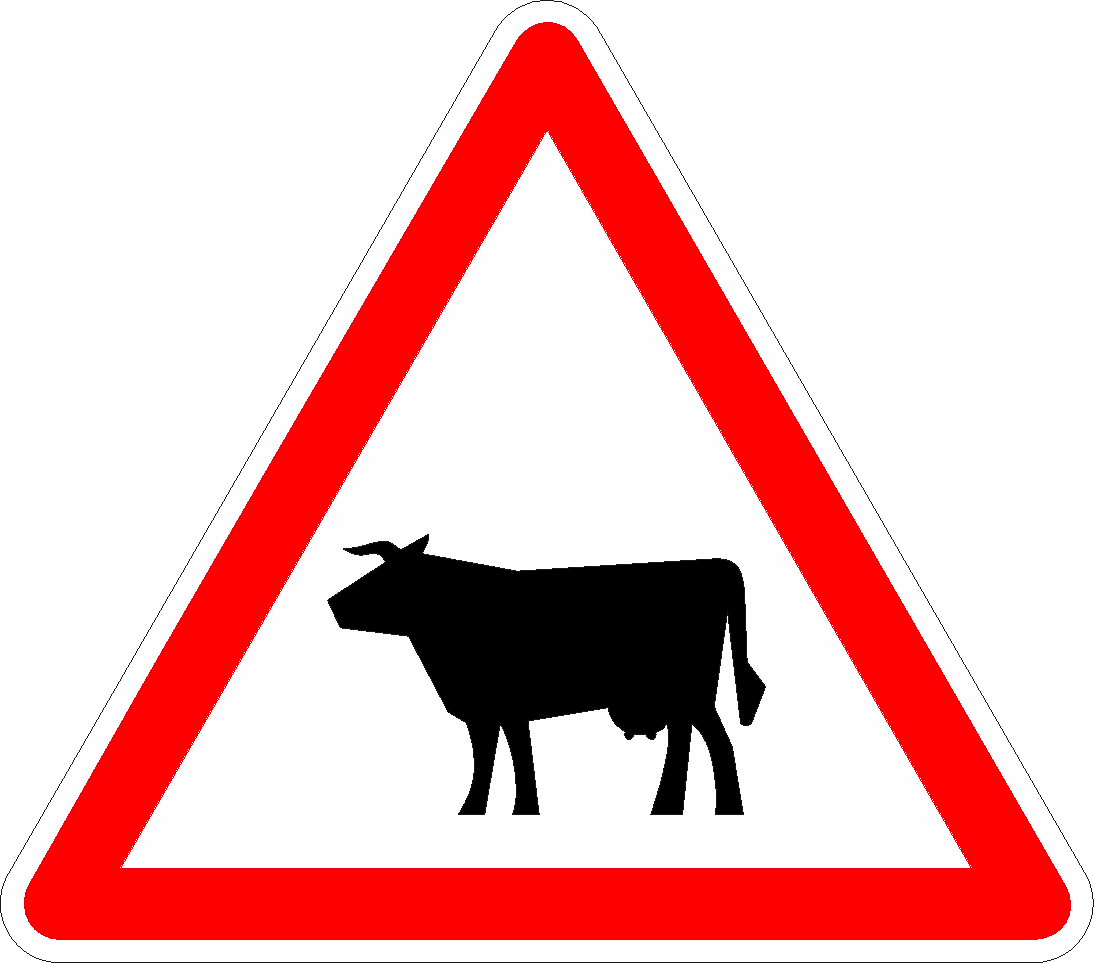
\includegraphics[height=2cm]{PanneauRouteA15a1.pdf}

\includegraphics[height=2cm]{PanneauRouteA15a2.pdf}

\includegraphics[height=2cm]{PanneauRouteA15b.pdf}

\includegraphics[height=2cm]{PanneauRouteA15c.pdf}

\includegraphics[height=2cm]{PanneauRouteA16.pdf}

\includegraphics[height=2cm]{PanneauRouteA17.pdf}

\includegraphics[height=2cm]{PanneauRouteA18.pdf}

\includegraphics[height=2cm]{PanneauRouteA19.pdf}

\includegraphics[height=2cm]{PanneauRouteA1a.pdf}

\includegraphics[height=2cm]{PanneauRouteA1b.pdf}

\includegraphics[height=2cm]{PanneauRouteA1c.pdf}

\includegraphics[height=2cm]{PanneauRouteA1d.pdf}

\includegraphics[height=2cm]{PanneauRouteA20.pdf}

\includegraphics[height=2cm]{PanneauRouteA21.pdf}

\includegraphics[height=2cm]{PanneauRouteA23.pdf}

\includegraphics[height=2cm]{PanneauRouteA24.pdf}

\includegraphics[height=2cm]{PanneauRouteA2a.pdf}

\includegraphics[height=2cm]{PanneauRouteA2b.pdf}

\includegraphics[height=2cm]{PanneauRouteA3.pdf}

\includegraphics[height=2cm]{PanneauRouteA3a.pdf}

\includegraphics[height=2cm]{PanneauRouteA3b.pdf}

\includegraphics[height=2cm]{PanneauRouteA4.pdf}

\includegraphics[height=2cm]{PanneauRouteA6.pdf}

\includegraphics[height=2cm]{PanneauRouteA7.pdf}

\includegraphics[height=2cm]{PanneauRouteA8.pdf}
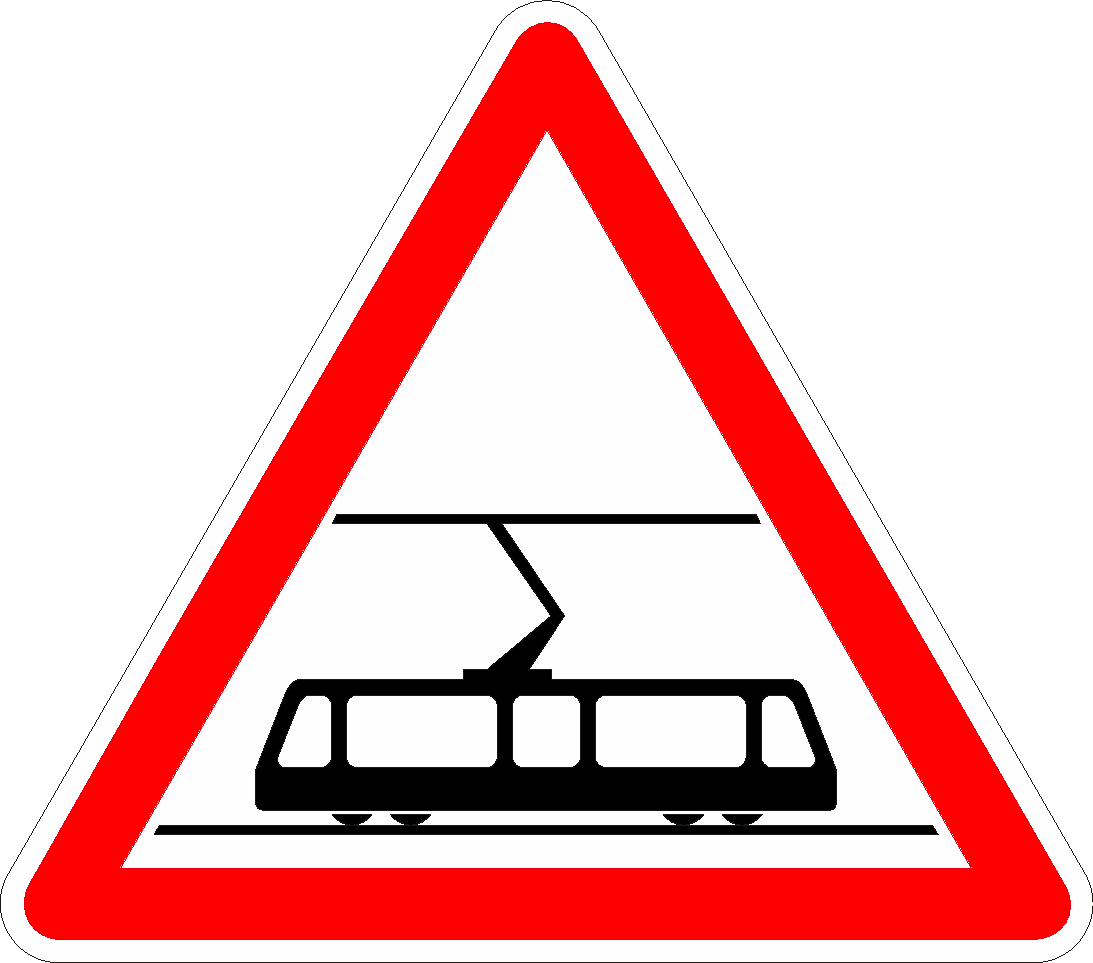
\includegraphics[height=2cm]{PanneauRouteA9.pdf}


\end{document}